\begin{figure}[hp]
	\centering
    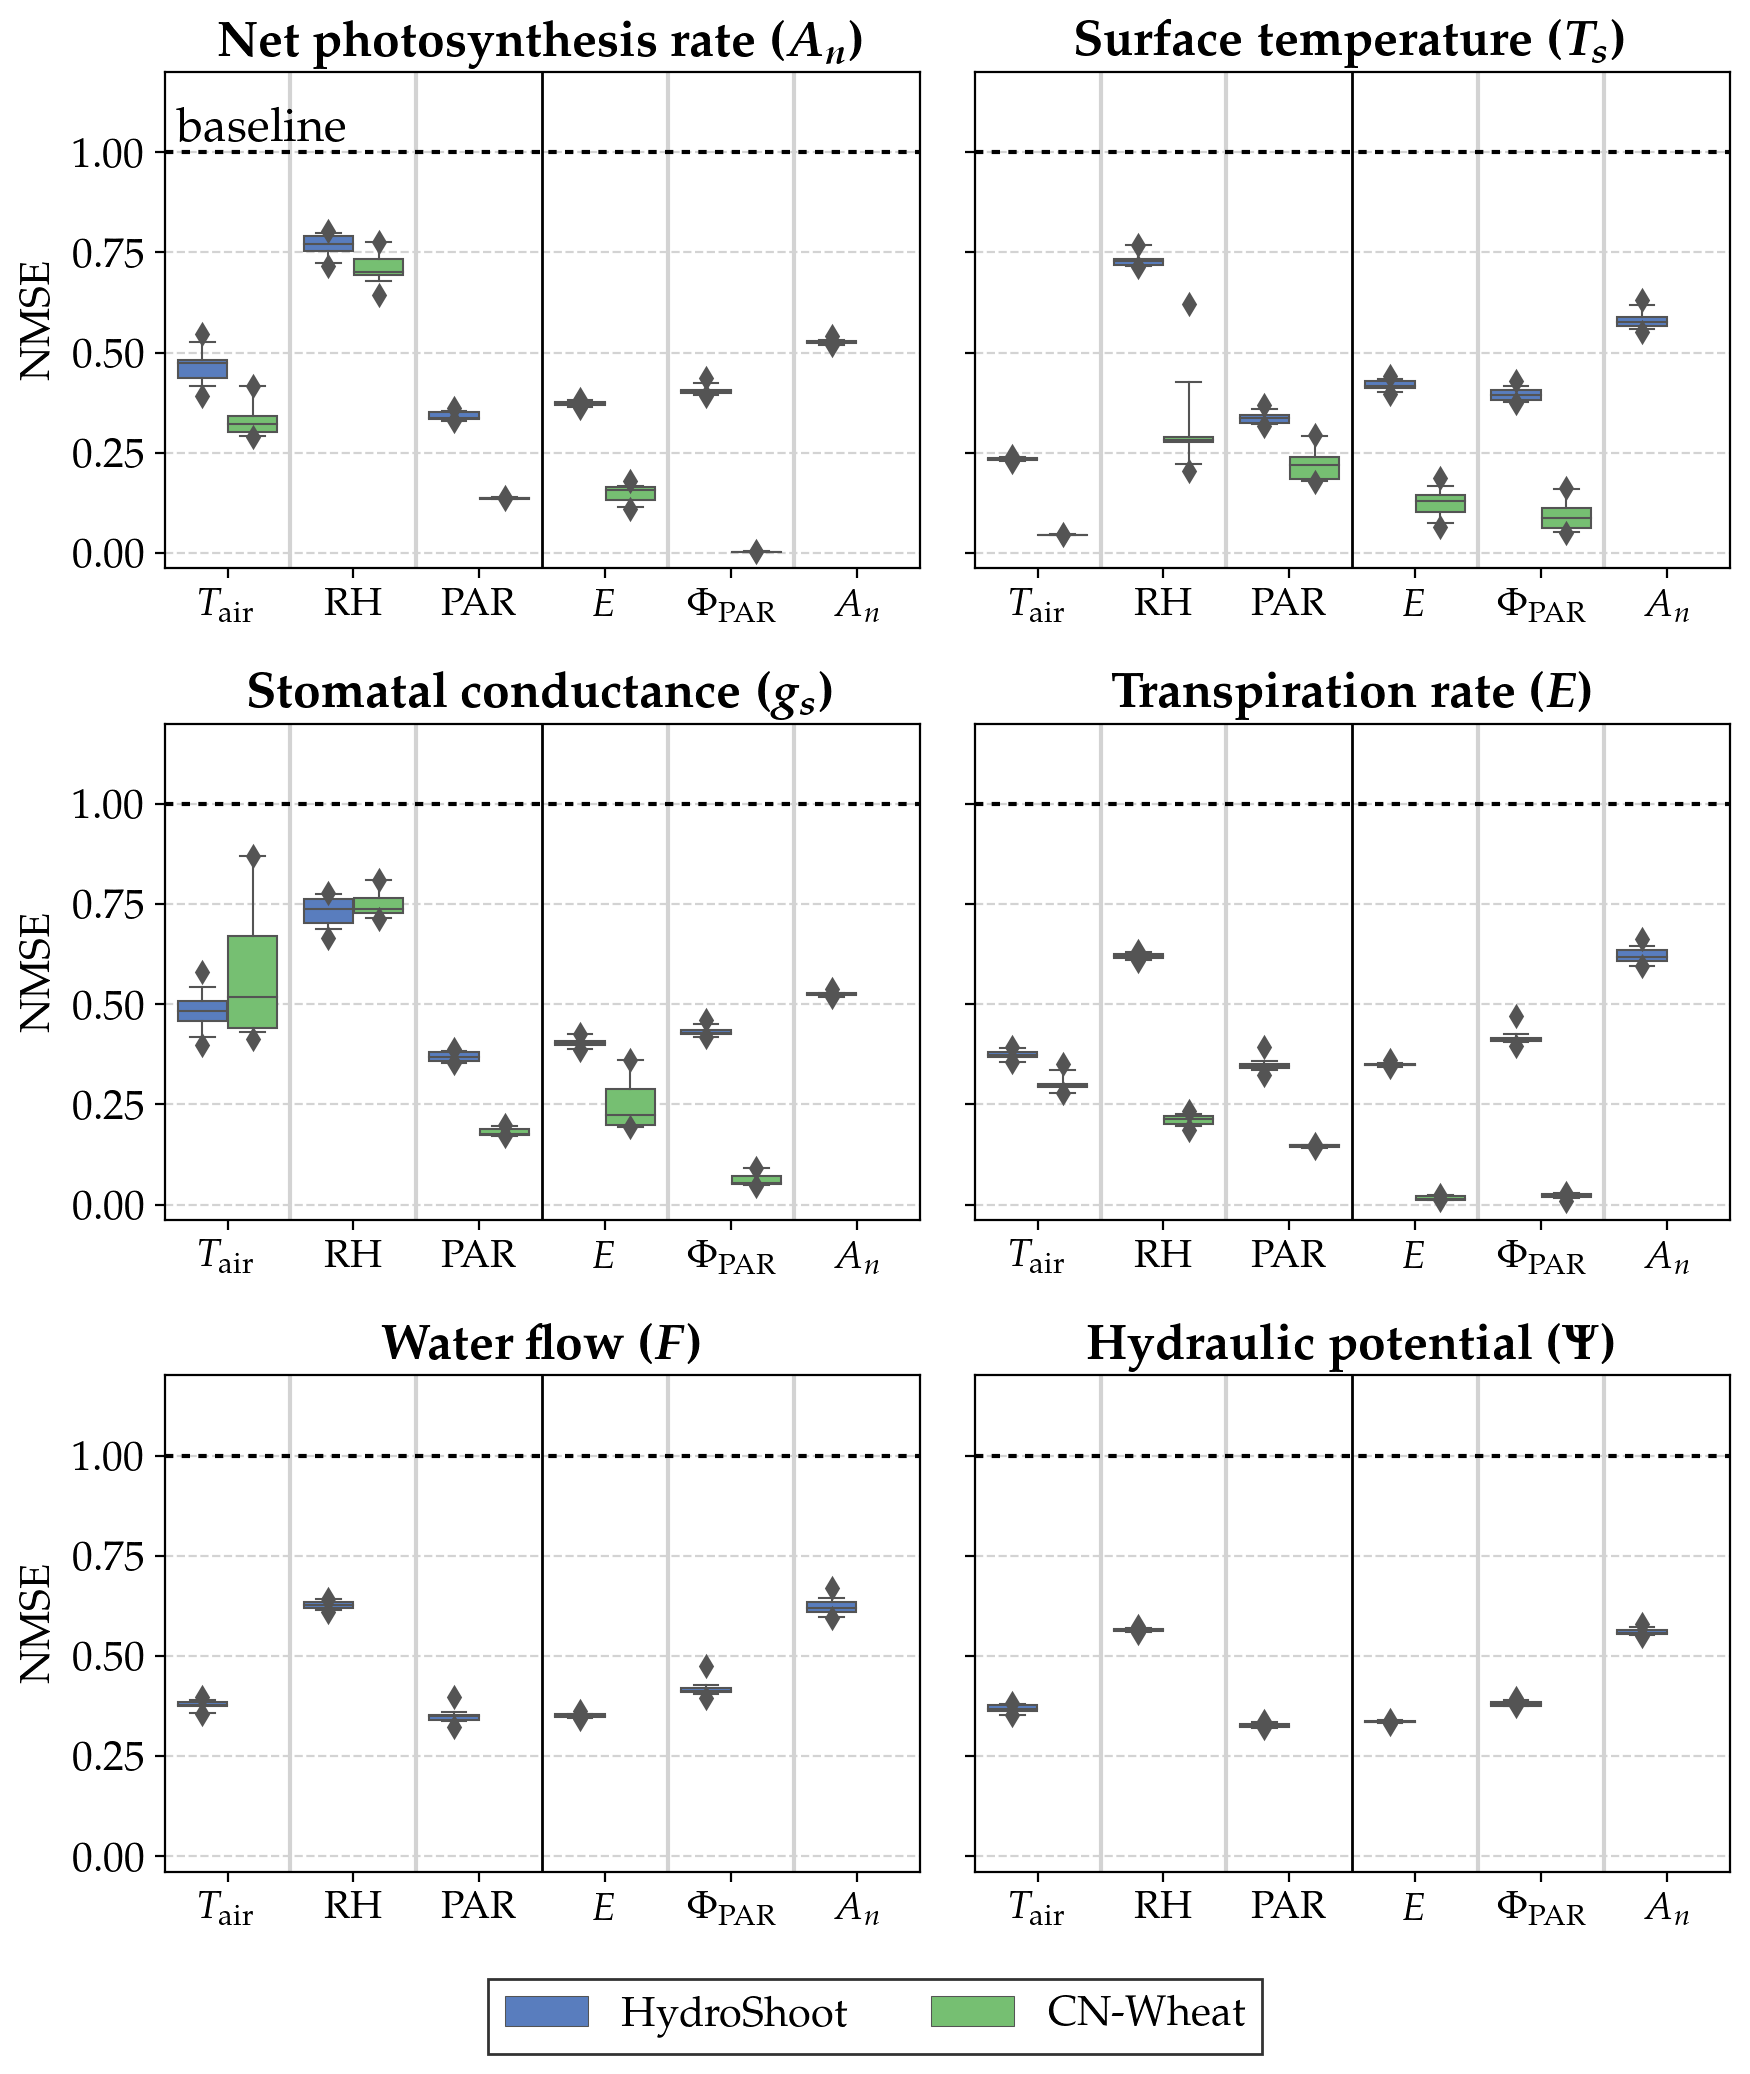
\includegraphics[width=0.82\textwidth]{img/regression_res_perf.png}
	\caption[Reservoir performance for input and physiological regression tasks.]
	        {Reservoir performance for input and physiological regression tasks.
	         The different plots show the prediction accuracy (y axis) for a suite of regression tasks (x axis) for each of the physiological reservoirs from \mbox{Table \ref{table:simulation_reservoirs}}.
	         The regression target of net photosynthesis rate  $A_n$ was only available for the HydroShoot model.
	         Each boxplot shows the distribution of test across 16 random reservoir samplings.
	         The box shows the quartiles of the distribution; the whiskers indicate the 5th and 95th percentiles.
	         Outliers are shown as a diamond shape.}
	\label{fig:input-phys-scores}
\end{figure}

% 	- *Caption:*
% 		- To measure the variance of the regression scores caused by the choice of observed plant elements, we used 16 random reservoir samplings and calculated
% - *Discussion boxplot figure:*
% - explanation of box plot whiskers etc.